%% ============================================================
%% Journal of Communication and Information Systems (JCIS)
%% Final version after the advisor's review and the source check
%% (IEEE Transactions two-column template).
%%
%% Compile with:  pdflatex -shell-escape -> bibtex -> pdflatex -shell-escape (x2)
%% Figures are SVG files included with the svg package (needs Inkscape).
%% Requires:      IEEEtran.cls, IEEEtran.bst, references.bib
%%
%% Comments "% [Item N]" refer to the advisor's numbered comments in
%% the annotated PDF; "% [E-mail N]" refers to his e-mail.
%% ============================================================
\documentclass[journal]{IEEEtran}

% ---- Math ----
\usepackage{amsmath,amssymb,amsfonts}
\usepackage{amsthm}
\usepackage{tikz}
\usetikzlibrary{positioning,arrows.meta}
\interdisplaylinepenalty=2500   % restore IEEEtran page breaks after amsmath

% ---- Algorithms ----
\usepackage{algorithm}
\usepackage{algorithmic}

% ---- Tables ----
\usepackage{array}
\usepackage{booktabs}

% ---- Figures ----
\usepackage{graphicx}
\usepackage{subcaption}
\usepackage[inkscapelatex=false]{svg}  % figures in SVG (compile with -shell-escape; requires Inkscape)

% ---- Misc ----
\usepackage{textcomp}
\usepackage{stfloats}
\usepackage{url}
\usepackage{cite}
\usepackage{xcolor}
\hyphenation{Lya-pu-nov non-li-near}


\begin{document}

% ============================================================
% TITLE AND AUTHORS (unchanged)
% ============================================================
\title{Analysis of the Chaotic Regime in the Filtered\\ H\'enon Map: Effect of FIR Filter Type\\ and Design Window}

\author{Kau\^e~de~Souza~Silva,
        Roger~Freitas~Pereira,
        Marcos~Felipe~Correa~Soares,
        Guilherme~Rodrigues~dos~Santos,
        and~Vin\'icius~da~Silva~Borges%
\thanks{K. de S. Silva is an undergraduate student in Computer Engineering
at the Faculdade Engenheiro Salvador Arena (FESA), Centro Educacional da
Funda\c{c}\~ao Salvador Arena, Estrada dos Alvarengas, 4001, S\~ao Bernardo
do Campo, SP, Brazil. ORCID: 0009-0009-1283-0996 (e-mail:
kaue.moelas.com@gmail.com).}%
\thanks{R. F. Pereira is an undergraduate student in Computer Engineering
at FESA, S\~ao Bernardo do Campo, SP, Brazil. ORCID: 0009-0000-5624-7422
(e-mail: roger\_freitas@live.com).}%
\thanks{M. F. C. Soares is an undergraduate student in Computer Engineering
at FESA, S\~ao Bernardo do Campo, SP, Brazil. ORCID: 0009-0009-9968-2227
(e-mail: marcosfelipe.soares2014@gmail.com).}%
\thanks{G. R. dos Santos is an undergraduate student in Computer Engineering
at FESA, S\~ao Bernardo do Campo, SP, Brazil. ORCID: 0009-0004-0281-8663
(e-mail: guilhermerodriguess130@gmail.com).}%
\thanks{V. da S. Borges is with the Computer Engineering Department, FESA,
S\~ao Bernardo do Campo, SP, Brazil. He is the academic advisor of this
work. ORCID: 0000-0001-5546-6842 (e-mail: viniciussbrg@gmail.com).}%
}

\markboth{Journal of Communication and Information Systems,~Vol.~XX, No.~X, Month~Year}%
{Silva \MakeLowercase{\textit{et al.}}: Analysis of the Chaotic Regime in the Filtered H\'enon Map}

\maketitle

% ============================================================
% ABSTRACT  [Items 1, 2, 3, 4]
% ============================================================
\begin{abstract}
The insertion of finite impulse response (FIR) filters in the feedback loop of
chaotic generators is a known strategy for bandwidth limitation in chaos-based
communication systems (CBCS). Although the filter does not prevent
master--slave synchronization, its interaction with the nonlinearity of the
generating map may destroy the chaotic behavior. This work investigates, by
numerical simulation, the conditions under which chaos is preserved in the
H\'enon map with an internal FIR filter, for four filter types (lowpass,
highpass, bandpass, and bandstop) and seven design windows, including a sweep of
the Kaiser shape parameter. Points of the plane formed by the filter order and
the cutoff frequency whose orbits become unbounded are classified as divergent.
The remaining points are classified as chaotic when the largest Lyapunov
exponent, which measures the average exponential rate at which nearby orbits
separate, exceeds a threshold of $5\times10^{-3}$, and as non-chaotic otherwise.
Filtering does not eliminate the chaotic regime but reorganizes it in a way that
depends on both the filter type and the window. Filters that remove the direct
current (DC) component make the fixed point of the map stable and yield no
chaotic point in the grid, whereas, for unit DC gain, the order, the cutoff frequency, and
the window decide the regime. At the orders studied, the designed filters do not
realize the nominal bandpass and bandstop masks, and the chaotic generators
confine their spectrum only partially. Therefore, neither the dynamics nor the
spectrum of a filtered generator follows from the filter specification, and
both must be verified for each design.
\end{abstract}

% [Item 5]
\begin{IEEEkeywords}
Chaos-based communication systems, H\'enon map,
FIR filters, window design, Lyapunov exponent.
\end{IEEEkeywords}

% ============================================================
\section{Introduction}\label{sec:intro}
% ============================================================
% [Items 6, 7, 8, 9] Paragraph 1: chaotic signals and their use as carriers
\IEEEPARstart{D}{eterministic} discrete-time chaotic signals are bounded in
amplitude, aperiodic, and exhibit sensitive dependence on initial conditions
(SDIC), so that orbits starting arbitrarily close separate, on average
exponentially fast~\cite{Alligood1996}. They also have a broadband spectrum
and a noise-like appearance, which motivates their use as carriers in
communication systems~\cite{Baptista2021}. Among the advantages usually
attributed to such carriers are the difficulty of interception by
unauthorized receivers, which places them among the physical-layer security
approaches~\cite{Mukherjee2014}, the spreading of the transmitted spectrum,
and robustness to multipath fading in some modulation
schemes~\cite{Kaddoum2016}. This
interest grew after Pecora and Carroll~\cite{Pecora1990} showed that two
identical chaotic systems can be synchronized despite SDIC, when the
receiver is driven by state variables of the transmitter.

% [Items 10, 11, 12] Paragraph 2: how a CBCS transmits information
In chaos-based communication systems (CBCS), the message is embedded in a
chaotic carrier at the transmitter and recovered at the receiver. In
coherent CBCS, the receiver synchronizes a replica of the transmitter
generator with the received signal and uses it to extract the message.
Non-coherent architectures, in contrast, recover the information from
statistical or structural properties of the received signal without a
synchronized replica~\cite{Kaddoum2016}. Examples of CBCS include chaotic
modulation schemes~\cite{Baptista2021}, image coding and
encryption~\cite{Sabatini2020}, systems based on three-dimensional
attractors~\cite{Souza2019}, and phase-locked loops for systems based on
chaotic attractors~\cite{Silva2025sbrt}.

% [Items 13--18] Paragraph 3: band limitation, filter in the loop, four types
The broadband spectrum of chaotic signals, however, conflicts with the fact
that practical channels are band-limited. If the spectrum of the transmitted
signal is not confined to the channel passband, the distortion introduced by
the channel prevents the receiver from synchronizing, and the message is
lost~\cite{Eisencraft2011}. To overcome this limitation, Eisencraft
\textit{et al.}~\cite{Eisencraft2009} proposed inserting a discrete-time
linear filter in the feedback loop of the chaotic generator, and Fontes and
Eisencraft~\cite{Fontes2016} showed that the filter does not prevent
synchronization, a result already indicated in~\cite{Eisencraft2009}.
Over band-limited channels, a filter in the feedback loop of the generator
allows coherent detection~\cite{Eisencraft2009,Fontes2016}.
Further practical limitations, such as finite-precision digital
implementation, were investigated by Borges and
Eisencraft~\cite{Borges2021sbrt}. The lowpass case corresponds to a baseband
channel, but other spectral masks arise in practice. Highpass filtering
removes the direct current (DC) component of the chaotic signal, which carries no information
and is blocked by capacitively coupled channels. Bandpass filtering confines the signal
to an allocated band, and bandstop filtering creates a spectral notch to
avoid narrowband interference or to coexist with other
systems~\cite{Li2013uwb}. From a dynamical standpoint, these four types also have different
gains at zero frequency, which determine the fixed point of the filtered
map~\cite{BorgesCNSNS2024}.

% [Items 19, 20] Paragraph 4: why the question is necessary and the gap
Inserting a filter in the feedback loop, however, changes the dynamics of the
generator, and nothing guarantees that the transmitted signal remains
chaotic. Once the unfiltered pair synchronizes, the filter preserves
synchronization for any choice of coefficients~\cite{BorgesTese2026}, but it
may destroy the chaotic behavior of the generator. Borges and Eisencraft
showed numerically that the coefficients determine whether the generated
signals are chaotic, periodic, or divergent, for a two-coefficient
filter~\cite{BorgesCSF2022} and for lowpass filters of increasing
order~\cite{Borges2022sbrt}, with bifurcation cascades, coexisting
attractors, crises, and shrimp-shaped periodic islands~\cite{Gallas1993}.
Borges \textit{et al.} extended this analysis to finite impulse response (FIR) filters with more
coefficients and different zero placements~\cite{BorgesCNSNS2024} and to
second-order all-pole filters~\cite{Borges2024sbrt}. The preservation of
chaos must therefore be verified for each filter design. It remains open
which combinations of filter type, design window, order, and cutoff
frequency keep the generator chaotic, and this is the question addressed
here.

% [Item 21] Paragraph 5: what this work does (single paragraph; the list of
% contributions was moved to Section V)
Previous studies varied the coefficients of a two-coefficient
filter~\cite{BorgesCSF2022}, the zero placement of the FIR
filter~\cite{BorgesCNSNS2024}, and the order and cutoff frequency of lowpass
filters designed with the Hamming and Blackman
windows~\cite{Borges2022sbrt,BorgesCNSNS2024}.
In practice, however, an FIR filter is specified by its frequency response
and designed by a method such as windowing, so the filter type and the design
window are natural design choices. This work investigates how these two
choices affect the preservation of chaos in the H\'enon map with an internal
FIR filter. Lowpass, highpass, bandpass, and bandstop filters are designed
with seven windows, including a sweep of the Kaiser shape
parameter~\cite{Kaiser1980}, and for each configuration the filter order and
the cutoff frequency are varied to build maps that classify the generated
signals as chaotic, non-chaotic, or divergent. The parameters of the H\'enon map
and the bandwidth of the bandpass and bandstop filters are kept fixed.

% Paragraph 6: organization of the paper (updated)
The remainder of this paper is organized as follows.
Section~\ref{sec:prelim} presents the preliminary concepts: the H\'enon map,
the H\'enon map with an FIR filter in the feedback loop, the largest Lyapunov
exponent, and the FIR design windows. Section~\ref{sec:method} describes the methodology,
Section~\ref{sec:results} presents and discusses the results, and
Section~\ref{sec:conclusion} summarizes the conclusions, the contributions of
the work, and future directions.

% ============================================================
% [E-mail 6] "Theoretical Background" -> "Preliminary Concepts"
\section{Preliminary Concepts}\label{sec:prelim}
% ============================================================
This section introduces the concepts needed to follow the rest of the paper.
The H\'enon map is presented first and then extended with an FIR filter in
the feedback loop. The largest Lyapunov exponent, used to classify the
signals generated by both systems, comes next, followed by the windows used
to design the filter.

% ---- II-A ----  [E-mail 7]: only the Hénon map, with a figure
\subsection{H\'enon Map}\label{sub:henon}
Consider the H\'enon map~\cite{Henon1976}
\begin{equation}
  \begin{cases}
    x_1(n+1) = \alpha - x_1^2(n) + \beta\, x_2(n), \\
    x_2(n+1) = x_1(n),
  \end{cases}
  \label{eq:henon}
\end{equation}
where $n\in\{0,1,2,\ldots\}$ is the discrete time, $x_1(n)$ and $x_2(n)$ are
the state variables, and $\alpha$ and $\beta$ are real parameters. Grouping
the state variables in the vector $\mathbf{x}(n)=[x_1(n)\;\,x_2(n)]^{T}$,
where $(\cdot)^{T}$ denotes transposition, \eqref{eq:henon} can be written
compactly as $\mathbf{x}(n+1)=\mathbf{F}(\mathbf{x}(n))$. The sequence of
states $\{\mathbf{x}(n)\}_{n\ge 0}$ obtained by iterating $\mathbf{F}$ from an
initial condition $\mathbf{x}(0)$ is called an \emph{orbit}~\cite{Alligood1996}.

Depending on the parameters and on the initial condition, an orbit may
converge to a fixed point, converge to a periodic orbit, behave chaotically,
or diverge~\cite{Alligood1996}. A \emph{fixed point} is a state
$\mathbf{x}^\star$ left unchanged by one iteration,
$\mathbf{x}^\star=\mathbf{F}(\mathbf{x}^\star)$, so that an orbit started at
$\mathbf{x}^\star$ stays there for all $n$. An orbit is \emph{bounded} when
there is a finite $M$ such that $\|\mathbf{x}(n)\|\le M$ for all $n$, and
\emph{divergent} otherwise~\cite{Alligood1996}. For \eqref{eq:henon}, the
condition $\mathbf{x}^\star=\mathbf{F}(\mathbf{x}^\star)$ gives two fixed
points, of which the positive one is used as the reference state in this
work.

Fig.~\ref{fig:henon} illustrates the chaotic and the periodic behaviors with
segments of $x_1(n)$ generated from two initial conditions that differ by
$10^{-3}$ in $x_2(0)$, as in~\cite{Borges2022sbrt}. In
Fig.~\ref{fig:henon}(a), with $\alpha=1.4$ and $\beta=0.3$, the signal is
aperiodic and, although the two initial conditions are nearly
indistinguishable, the distance between them first exceeds $0.1$ at $n=11$
and reaches order one at $n=18$; this is the SDIC of chaotic signals. In Fig.~\ref{fig:henon}(b),
with $\alpha=0.9$ and $\beta=0.3$, both orbits converge to the same period-2
orbit, which alternates between $x_1\approx1.08$ and $x_1\approx-0.38$, and
the difference between the initial conditions is lost.
Throughout this work, $\alpha=1.4$ and $\beta=0.3$ are adopted.

\begin{figure}[!t]
\centering
\includesvg[width=\columnwidth]{Figures/fig_henon_signals}
\caption{Segments of $x_1(n)$ obtained from \eqref{eq:henon} with
$x_1(0)=x_2(0)=0$ (solid blue) and $x_1(0)=0$, $x_2(0)=0.001$ (dashed red).
(a)~$\alpha=1.4$, $\beta=0.3$: chaotic signal. (b)~$\alpha=0.9$, $\beta=0.3$:
periodic signal (period~2).}
\label{fig:henon}
\end{figure}

% ---- II-B ----  [E-mail 8]: expanded system with the FIR filter
\subsection{H\'enon Map With an FIR Filter in the Feedback Loop}\label{sub:expanded}


This subsection defines the filter, the expanded system obtained when the
filter is inserted in the map, and the quantities of that system used in the
rest of the paper. To limit the bandwidth of the generated signal, Eisencraft
\textit{et al.}~\cite{Eisencraft2009} and Fontes and
Eisencraft~\cite{Fontes2016} proposed filtering $x_1(n)$ with an FIR filter and feeding the filter output back into the
map. Fig.~\ref{fig:generator} shows the generator studied in this work. The output of the filter is
\begin{equation}
  x_3(n) = \sum_{j=0}^{N_s-1} c_j\, x_1(n-j),
  \label{eq:filtro}
\end{equation}
where $c_j$, $0\le j\le N_s-1$, are the $N_s$ filter coefficients. The filter
order is $N_z=N_s-1$, equal to the number of zeros of the transfer function
obtained by taking the $z$-transform of~\eqref{eq:filtro} with zero initial
conditions~\cite{Oppenheim2009},
\begin{equation}
  H(z)=\frac{X_3(z)}{X_1(z)}=\sum_{j=0}^{N_s-1} c_j\, z^{-j}.
  \label{eq:tf}
\end{equation}

\begin{figure}[!t]
\centering
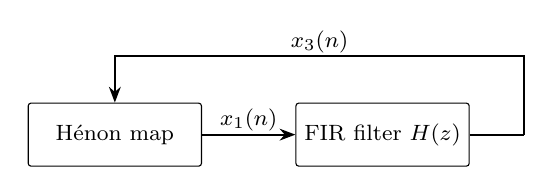
\begin{tikzpicture}[font=\footnotesize,
  blk/.style={draw, rounded corners=1pt, minimum width=2.2cm, minimum height=0.8cm, inner sep=2pt, align=center},
  io/.style={inner sep=1pt},
  ar/.style={-{Stealth[length=2mm]}, thick}]
  \node[blk] (henon) at (0,0) {Hénon map};
  \node[blk] (fir) at (3.4,0) {FIR filter $H(z)$};
  \coordinate (J) at (5.2,0);
  \draw[ar] (henon) -- node[above,io] {$x_1(n)$} (fir);
  \draw[thick] (fir.east) -- (J);
  \draw[ar] (J) -- (5.2,1.0) -- (0,1.0) -- (henon.north);
  \node[io] at (2.6,1.0) [above] {$x_3(n)$};
\end{tikzpicture}
\caption{Generator studied in this work, described by~\eqref{eq:expandido}.}
\label{fig:generator}
\end{figure}

Evaluating $H(z)$ on the unit circle, $z=e^{j\omega}$, gives the frequency
response $H(e^{j\omega})$, where $\omega\in[0,\pi]$ is the normalized angular
frequency in rad/sample. The frequency response fixes the passband, the
transition width, and the stopband attenuation delivered by a given set of
coefficients~\cite{Oppenheim2009}. In this work, it is specified by the filter
type (lowpass, highpass, bandpass, or bandstop) and by a cutoff frequency
$\omega_c$. Its value at $\omega=0$ is the DC gain of the filter,
$G=H(e^{j0})=\sum_{j}c_j$~\cite{Oppenheim2009}.

The filtered signal $x_3(n)$ replaces $x_1(n)$ in the nonlinear term
of~\eqref{eq:henon}. Because~\eqref{eq:filtro} depends on the past samples
$x_1(n-1),\ldots,x_1(n-N_s+1)$, the pair $(x_1,x_2)$ is no longer a complete
state of the system. These samples are therefore stored as auxiliary state
variables $x_4,\ldots,x_{N_s}$, each holding a one-step delay of the
preceding one. For $N_s\ge3$, the resulting expanded system
is~\cite{Borges2022sbrt,BorgesCNSNS2024}
\begin{equation}
  \begin{cases}
    x_1(n+1) = \alpha - x_3^2(n) + \beta\, x_2(n), \\
    x_2(n+1) = x_1(n), \\
    x_3(n+1) = c_0\bigl(\alpha - x_3^2(n) + \beta\, x_2(n)\bigr) + c_1\, x_1(n) \\
    \qquad\qquad + c_2\, x_2(n) + c_3\, x_4(n) + \cdots + c_{N_s-1}\, x_{N_s}(n), \\
    x_4(n+1) = x_2(n), \\
    x_j(n+1) = x_{j-1}(n),\quad j = 5,\ldots,N_s,
  \end{cases}
  \label{eq:expandido}
\end{equation}
whose dimension is $K=N_s$; for $N_s=3$, the terms in $x_4,\ldots,x_{N_s}$
are absent. For $N_s\le2$, the filter output $x_3(n)=c_0x_1(n)+c_1x_2(n)$ (with
$c_1=0$ for $N_s=1$) is a function of the current state, so no auxiliary
variable is needed and the system keeps dimension $K=2$:
\begin{equation}
  \begin{cases}
    x_1(n+1) = \alpha - \bigl(c_0x_1(n)+c_1x_2(n)\bigr)^2 + \beta\, x_2(n), \\
    x_2(n+1) = x_1(n).
  \end{cases}
  \label{eq:expandido2}
\end{equation}
For $N_s=1$ and $c_0=1$, the filter is the identity and the original
map~\eqref{eq:henon} is recovered. As for~\eqref{eq:henon}, the fixed points of~\eqref{eq:expandido} are the
solutions of $\mathbf{x}^\star=\mathbf{F}(\mathbf{x}^\star)$, where
$\mathbf{F}$ now denotes the right-hand side of~\eqref{eq:expandido}. At a
fixed point all delayed samples are equal, $x_1=x_2=x_4=\cdots=x_{N_s}=p$, and
$x_3=Gp$, which gives $G^2p^2+(1-\beta)p-\alpha=0$~\cite{BorgesCNSNS2024,BorgesTese2026}.
Its positive root is
\begin{equation}
  p = \frac{2\alpha}{(1-\beta)+\sqrt{(1-\beta)^2+4\alpha G^2}}.
  \label{eq:pfixo}
\end{equation}
For $G = 0$, approximately the case of highpass and bandpass filters,
$p = \alpha/(1-\beta)$. The
positive fixed point of the expanded system is
$\mathbf{x}^\star=[p\;\,p\;\,Gp\;\,p\cdots p]^T$ (or
$[p\;\,p]^T$ for $N_s\le2$); it depends on the filter only through its DC
gain $G$ and is used to initialize the simulations
(Section~\ref{sub:estimator}).

% ---- II-C ----  [E-mail 9, second]: largest Lyapunov exponent
% (adapted from Borges and Eisencraft, SBrT 2022, Sec. III)
\subsection{Largest Lyapunov Exponent}\label{sub:lyap}
The sensitivity of a system to its initial conditions can be quantified by
how fast two very close states move apart as they evolve. Lyapunov proposed
measuring this separation under the assumption that it grows exponentially,
so that the Lyapunov exponent is the natural logarithm of the average rate at
which two nearby orbits separate~\cite{Alligood1996,Borges2022sbrt}. An
exponent equal to $\ln2$ along a given direction, for instance, means that the
distance between the orbits doubles, on average, at each iteration in that
direction, whereas a negative exponent means that the orbits approach each
other. The SDIC of a chaotic signal is therefore measured by the Lyapunov
exponent: a computationally generated signal that is bounded, aperiodic, and
has at least one positive Lyapunov exponent is chaotic~\cite{Alligood1996}.

A map of dimension $K$ has $K$ Lyapunov exponents, one for each direction of
the state space, denoted in decreasing order by
$\lambda_1\ge\lambda_2\ge\cdots\ge\lambda_K$. They are computed from the
\emph{Jacobian matrix} $\mathbf{J}(n)$, the $K\times K$ matrix of partial
derivatives $[\mathbf{J}(n)]_{ik}=\partial F_i/\partial x_k$ evaluated at
$\mathbf{x}(n)$, which describes how a small perturbation of the state is
transformed in one iteration~\cite{Alligood1996}. For the expanded
system~\eqref{eq:expandido}, it is~\cite{Borges2022sbrt,BorgesCNSNS2024}
\begin{equation}
  \mathbf{J}(n) = \begin{pmatrix}
    0 & \beta & -2x_3(n) & 0 & \cdots & 0 \\
    1 & 0 & 0 & 0 & \cdots & 0 \\
    c_1 & c_0\beta + c_2 & -2c_0 x_3(n) & c_3 & \cdots & c_{N_s-1} \\
    0 & 1 & 0 & 0 & \cdots & 0 \\
    \vdots & & & \ddots & & \vdots \\
    0 & \cdots & 0 & 0 & 1 & 0
  \end{pmatrix},
  \label{eq:jacobiana}
\end{equation}
in which only the third row depends on the filter coefficients; for
$N_s\le2$, $\mathbf{J}(n)$ is the $2\times2$ Jacobian
of~\eqref{eq:expandido2}. For the map~\eqref{eq:henon}, $\det\mathbf{J}(n)=-\beta$
for every $n$, so its two exponents satisfy
$\lambda_1+\lambda_2=\ln|\beta|$~\cite{Alligood1996}, an identity used in
Section~\ref{sub:validation} to validate the implementation.

The exponents are computed by the tangent-map
method~\cite{Alligood1996,Borges2022sbrt}. A hypersphere of unit radius
centered at $\mathbf{x}(0)$ is represented by a matrix $\mathbf{U}$ whose
columns are its orthogonal axes. Each iteration of the map turns the
hypersphere into an ellipsoid, and after $n$ iterations the axes of the
ellipsoid are the columns of
$\mathbf{J}(n-1)\cdots\mathbf{J}(1)\mathbf{J}(0)\mathbf{U}$. Computing the
lengths of these axes directly is numerically inadequate, because directions
that are stretched and directions that are compressed produce very large and
very small numbers. Instead, the growth of each axis is computed at every
iteration, and the axes are orthonormalized again before the next one, in the
following steps~\cite{Alligood1996}:
\begin{enumerate}
  \item Choose an orthonormal basis $\{\mathbf{w}_1(0),\ldots,\mathbf{w}_K(0)\}$
  and compute $\mathbf{z}_k(0)=\mathbf{J}(0)\mathbf{w}_k(0)$, $1\le k\le K$.
  These vectors are axes of the new ellipsoid, but they are not necessarily
  orthogonal.
  \item Orthogonalize them by the Gram--Schmidt process,
  \begin{equation}
    \mathbf{y}_k(1)=\mathbf{z}_k(0)-\sum_{i=1}^{k-1}
    \frac{\mathbf{z}_k(0)\cdot\mathbf{y}_i(1)}{\|\mathbf{y}_i(1)\|^2}\,
    \mathbf{y}_i(1),
    \label{eq:gs}
  \end{equation}
  where ``$\cdot$'' denotes the scalar product.
  \item Normalize the vectors, $\mathbf{w}_k(1)=\mathbf{y}_k(1)/\|\mathbf{y}_k(1)\|$,
  which gives the orthonormal basis for the next iteration.
  \item Apply the Jacobian at the next point of the orbit,
  $\mathbf{z}_k(1)=\mathbf{J}(1)\mathbf{w}_k(1)$, and repeat steps~2 and~3.
  After $n$ repetitions, the vectors $\mathbf{y}_k(1),\ldots,\mathbf{y}_k(n)$
  are available.
\end{enumerate}
The Lyapunov exponent in the $k$-th direction is then
\begin{equation}
  \lambda_k = \lim_{n\to\infty}
  \frac{\ln\|\mathbf{y}_k(1)\| + \cdots + \ln\|\mathbf{y}_k(n)\|}{n}.
  \label{eq:lyap}
\end{equation}

Only the largest exponent, $\lambda_1$, is used in this work. For
$\alpha=1.4$ and $\beta=0.3$, the map
\eqref{eq:henon} has
$\lambda_1\approx0.42$~\cite{Sprott2003}.

Based on these concepts, each orbit is classified as
\begin{equation}
  \begin{cases}
    \text{divergent}, & \text{if the orbit is unbounded},\\
    \text{chaotic},   & \text{if it is bounded and } \lambda_1 > \theta, \\
    \text{non-chaotic}, & \text{if it is bounded and } \lambda_1 \le \theta,
  \end{cases}
  \label{eq:criterio}
\end{equation}
where $\theta=5\times10^{-3}$ is the classification threshold. The
non-chaotic class also includes convergence to a fixed point, because
the criterion distinguishes only the presence or absence of chaos and not the
period of the limit orbit. The numerical detection of unbounded orbits is
described in Section~\ref{sub:metrics}.

% ---- II-D ----  [E-mail 9]: design windows
\subsection{FIR Design Windows}\label{sub:windows}
This subsection describes how the coefficients $c_j$ are obtained and which
design windows are compared. The coefficients are obtained by the window
method~\cite{Oppenheim2009,Harris1978}: the impulse response of the ideal
filter, which is infinitely long, is conveniently delayed and truncated by a
window of $N_s$ samples. The shape of the window sets a trade-off between the
stopband attenuation and the width of the transition band of the resulting
filter: windows with lower side lobes give higher attenuation at the cost of
a wider transition band~\cite{Harris1978}.

Seven windows are considered (Table~\ref{tab:windows}). The values listed
are the peak side-lobe levels of the discrete-time Fourier transform of each
window, relative to the main-lobe peak~\cite{Harris1978}; in the window
method, lower side lobes give higher stopband attenuation of the designed
filter~\cite{Oppenheim2009}. The values range from $-13$~dB for the
rectangular window, whose abrupt truncation produces strong side lobes, to
$-92$~dB for the four-term Blackman--Harris window, whose cosine-sum
coefficients are chosen to cancel side lobes~\cite{Harris1978}.

\begin{table}[!t]
\caption{FIR Windows Evaluated and Their Peak Side-Lobe Levels\label{tab:windows}}
\centering
\begin{tabular}{lc}
\toprule
\textbf{Window} & \textbf{Side lobe (dB)} \\
\midrule
Rectangular (boxcar)          & $-13$    \\
Bartlett                      & $-27$    \\
Hann                          & $-32$    \\
Hamming                       & $-43$    \\
Blackman                      & $-58$    \\
Blackman--Harris              & $-92$    \\
Kaiser ($\beta_K$ variable)   & variable \\
\bottomrule
\end{tabular}

\vspace{2pt}
{\footnotesize Source: adapted from~\cite{Harris1978}.}
\end{table}

The seven windows cover a broad range of this trade-off: the rectangular
window as the worst case; the Bartlett and Hann windows as classical
intermediate cases; the Hamming window, adopted as a reference because it was
used in the previous works on the filtered H\'enon
map~\cite{Fontes2016,Borges2022sbrt}; and the Blackman and Blackman--Harris
windows as high-attenuation cases. The Kaiser
window~\cite{Kaiser1980} has a shape parameter $\beta_K\ge0$ that varies the
trade-off continuously without changing the filter order: for
$\beta_K\in[0.5,20]$ its peak side-lobe level, computed here for a window of
101 samples, goes from about $-13.6$~dB to $-155$~dB, a range that contains
the side-lobe levels of the Bartlett, Hann, Hamming, Blackman, and
Blackman--Harris windows in Table~\ref{tab:windows}, and for $\beta_K=0$ the
window reduces to the rectangular one. The sweep of $\beta_K$ therefore
provides a continuous path between the fixed windows. Values $\beta_K>12$
correspond to stopband attenuations above about 120~dB~\cite{Oppenheim2009},
beyond practical requirements; they are included to locate the maximum of the
chaotic coverage (Section~\ref{sub:beta}).

% ---- II-E ----  Motivation: synchronization versus chaos (former II-B),
% condensed; terms adjusted as requested in Item 19.
\section{Methodology}\label{sec:method}
% ============================================================
The research adopts a quantitative-experimental approach: for each filter
design, the expanded system~\eqref{eq:expandido} is simulated, $\lambda_1$ is
estimated, and each grid point is classified by~\eqref{eq:criterio}. All simulations were implemented in the open-source package
\texttt{chaotic\_pfc} (BSD-3-Clause license)~\cite{chaoticPFC2026}; the 184
sweeps took about 10 min on a four-core laptop.

% ---- III-A ----  (former III-B and III-C)
\subsection{Filter Types and Parameter Grid}\label{sub:grid}
Four filter types are designed with the seven windows of
Table~\ref{tab:windows} by the routine \texttt{firwin} of the SciPy
library~\cite{Virtanen2020}. For lowpass and highpass filters, $\omega_c$ is
the cutoff frequency; for bandpass and bandstop filters, it is the center of a
band of fixed total width $\Delta\omega=0.05\,\pi$, placed symmetrically around
$\omega_c$. Near the ends of the grid, the band edges are clipped to the interval
$(0,1)$ of $\omega/\pi$, so the band is narrower and asymmetric for the cutoff
values closest to $0$ and to $1$. On the normalized axis $\omega/\pi\in(0,1)$, this width is $5\%$
of the range and spans about five steps of the cutoff grid. This
$\Delta\omega=0.05\,\pi$ is nominal: at the orders of the grid, the realized
filter is much wider for bandpass and barely rejects the band for bandstop
(for a band centered at $\omega_c=0.5\pi$, with the six fixed windows at
$N_z=10$, the realized bandpass 3\,dB width is between $0.18\,\pi$ and
$0.38\,\pi$ and the bandstop attenuation at the band center between $0.70$ and
$2.04$\,dB; at $N_z=40$, only the rectangular window among the fixed windows
reaches 20\,dB, whereas the others stay below 6.2\,dB). Fixing $\Delta\omega$ also isolates
the effect of $\omega_c$; the width is left as a variable for future work
(Section~\ref{sec:conclusion}).

Because it is the frequency response, and not the individual coefficients,
that must be matched to the channel, the sweep
variables are the filter order $N_z$ and the cutoff frequency $\omega_c$. For
lowpass and bandpass filters, $N_z\in\{1,2,\ldots,40\}$ and 100 values of
$\omega_c/\pi$ linearly spaced from $10^{-5}$ to $1-10^{-5}$ are swept, giving
$4{,}000$ grid points per window--filter configuration. For highpass and
bandstop filters, the parity restriction of the window method requires even
$N_z$~\cite{Oppenheim2009}, because a filter with an odd order has a forced
zero at $\omega=\pi$, which a passband that includes $\omega=\pi$ does not
allow; thus
$N_z\in\{2,4,\ldots,40\}$, with $2{,}000$ points per configuration. The six
fixed windows give $4\times6=24$ configurations, and the Kaiser window is
swept over 40 values of $\beta_K\in[0.5,20.0]$, with step $0.5$, for the four
filter types, adding 160 configurations, for a total of 184 sweeps and
$552{,}000$ grid points. The case $\beta_K=0$, which coincides with the
rectangular window, was also swept as a check and reproduced the rectangular
configurations exactly; it is not counted separately. For the Hann and Bartlett windows with lowpass and
bandpass filters, \texttt{firwin} returns non-finite coefficients for $N_z=1$, because the
symmetric two-sample windows are zero; these 100 points per configuration are
classified as divergent because of the filter design, not of the map dynamics.

% ---- III-B ----  (former III-D and III-E)
\subsection{Lyapunov Estimator and Initial Conditions}\label{sub:estimator}
Computing all $K$ exponents by the method of Section~\ref{sub:lyap} costs
$\mathcal{O}(K^3)$ operations per iteration, dominated by the Gram--Schmidt
orthogonalization. As in~\cite{BorgesCNSNS2024}, $\lambda_1$ is taken as the
largest of the $K$ finite-time exponents. To reduce the cost, the sweeps first
propagate a single tangent vector, multiplied by $\mathbf{J}(n)$ at each
iteration and renormalized once every ten iterations, which costs
$\mathcal{O}(K)$ per iteration (Algorithm~\ref{alg:lyap}); the formulation
follows Wolf \textit{et al.}~\cite{Wolf1985}, and the renormalization period
follows Benettin \textit{et al.}~\cite{Benettin1980a,Benettin1980b}. Grid points whose mean estimate lies within $5\times10^{-3}$ of the threshold
$\theta$ of (\ref{eq:criterio}), that is, $|\lambda_1-\theta|<5\times10^{-3}$,
are recomputed with the full spectrum, using the modified Gram--Schmidt
algorithm; 23,000 of the 552,000 grid points (4.17\%) were recomputed. The first
direction of the full-spectrum computation follows the same path as the single
tangent vector, so the recomputation changes the estimate only when another
direction has a larger finite-time exponent.

\begin{algorithm}[!t]
\caption{Single-vector estimation of $\lambda_1$ with periodic renormalization.}\label{alg:lyap}
\begin{algorithmic}[1]
\STATE \textbf{Input:} initial condition $\mathbf{x}_0$; burn-in iterations $N_{\text{burn}}$; accumulation cap $N_{\text{map}}$; tolerance $\varepsilon$.
\STATE $\mathbf{w}\leftarrow[1\;0\;\cdots\;0]^T$;\; $s\leftarrow 0$;\; $\mathbf{x}\leftarrow\mathbf{x}_0$.
\FOR{$i=1$ \TO $N_{\text{burn}}$}
  \STATE $\mathbf{x}\leftarrow\mathbf{F}(\mathbf{x})$ \quad(discard transient)
  \IF{$\mathbf{x}$ is non-finite}
    \STATE \textbf{return} DIVERGENT \quad(grid point)
  \ENDIF
\ENDFOR
\FOR{$i=1$ \TO $N_{\text{map}}$}
  \STATE $\mathbf{w}\leftarrow\mathbf{J}(\mathbf{x})\,\mathbf{w}$ \quad(tangent-vector evolution at the current state)
  \STATE $\mathbf{x}\leftarrow\mathbf{F}(\mathbf{x})$ \quad(orbit evolution)
  \IF{$\mathbf{x}$ is non-finite}
    \STATE \textbf{return} NaN \quad(divergent orbit)
  \ENDIF
  \IF{$i$ is a multiple of 10}
    \STATE $r\leftarrow\|\mathbf{w}\|$;\; $s\leftarrow s+\ln\max(r,10^{-300})$;\; if $r>10^{-300}$ then $\mathbf{w}\leftarrow\mathbf{w}/r$
    \STATE every 100 iterations with $i\ge500$: stop if $s/i$ varied less than $\varepsilon$ in two consecutive checks
  \ENDIF
\ENDFOR
\STATE \textbf{return} $\lambda_1=s/i$
\end{algorithmic}
\end{algorithm}

Accumulation stops early when the estimate of $\lambda_1$ varies less than the
tolerance $\varepsilon=10^{-3}$ in two consecutive checks, made every 100
iterations after the 500th. Requiring two checks avoids premature stops in
windows of chaotic intermittency, in which $\lambda_1$ oscillates for hundreds
of iterations before stabilizing.

For each grid point $(N_z,\omega_c)$, $N_{\text{IC}}=25$ initial conditions are
drawn near the positive fixed point $\mathbf{x}^\star$ of the expanded system
(Section~\ref{sub:expanded}): each component is $x_k^\star+0.1\,u$, with
$u\sim U[0,1)$. For each initial condition,
$N_{\text{burn}}=500$ iterations are discarded as transient, and $\lambda_1$ is
accumulated for at most $N_{\text{map}}=3{,}000$ iterations. The value
assigned to the grid point is the mean of $\lambda_1$ over the initial
conditions.

The value $N_{\text{burn}}=500$ is much longer than the transients of the
unfiltered map and accommodates longer transients near bifurcation
boundaries, although not all of them (Section~\ref{sub:ranking}). The value $N_\text{map}$ acts as a cap: with early stopping, the median number
of accumulated iterations per configuration lies between 700 and 1,200, with a
floor of 700, and the mean horizon reaches the cap at only 6 of the 552,000 grid
points. In all experiments,
$\alpha=1.4$, $\beta=0.3$,
and the seed of the pseudo-random generator is 42.

% ---- III-C ----  (former III-F)
\subsection{Classification and Chaotic-Coverage Metrics}\label{sub:metrics}
Each grid point is classified by~\eqref{eq:criterio}. Numerically, an orbit is
taken as unbounded when its state becomes non-finite (NaN or infinity); from
that iteration on, every term of~\eqref{eq:lyap} is non-finite, so the
simulation can be stopped. The divergence rule has three steps. First, the
estimator returns a non-finite value for an initial condition as soon as its
state becomes non-finite. Second, a grid point is divergent when at least one
of its 25 initial conditions becomes non-finite during the burn-in. Third, an
initial condition that becomes non-finite only after the burn-in is
discarded, and the value of the grid point is the mean of $\lambda_1$ over the
remaining initial conditions. This step differs from~\cite{BorgesCNSNS2024}, in
which a grid point is divergent when any of its initial conditions becomes
non-finite. Points with non-finite filter coefficients
(Section~\ref{sub:grid}) are also divergent.




The threshold $\theta=5\times10^{-3}$ in (\ref{eq:criterio}) separates two
populations of finite-time estimates. Over the 184 sweeps, 13{,}068 of
the 54{,}470 grid points with a positive estimate lie in $(0,10^{-3}]$,
whereas bins of width $10^{-3}$ between $5\times10^{-3}$ and $2\times10^{-2}$
hold between 400 and 516 points each. The first population
is consistent with quasi-periodic orbits, whose exponent is zero but whose
finite-time estimate decays as $1/N$ with the number $N$ of iterations: for 30
lowpass points with $N_z=3$ and $0<\lambda_1\le\theta$, recomputed with
$N=3\times10^3$, $3\times10^4$, and $3\times10^5$, 18 kept a positive estimate
at all horizons, with a median log--log slope of $-0.96$, and the other 12
changed sign.

Let $N_{\text{grid}}$ be the number of grid points of a configuration, $N_b$
the number of bounded (chaotic or non-chaotic) points, and $N_c$ the number of
chaotic points. The \emph{conditional} fraction
$\rho_c^{\text{cond}}=N_c/N_b$ is the share of chaotic points among the bounded
ones; it measures the tendency to chaos once divergence is excluded and is
relevant when $N_z$ and $\omega_c$ can be adjusted to reach a non-divergent
operating point. The \emph{absolute} fraction
$\rho_c^{\text{abs}}=N_c/N_{\text{grid}}$ is the share of the whole design
space that yields a chaotic generator and is relevant when a broad operating
range is sought. Using fractions also makes the comparison between filter
types independent of their different grid sizes (Section~\ref{sub:grid}).

% ---- III-D ----  (former III-G)
\subsection{Statistical Treatment}\label{sub:stats}
Two levels are kept separate. At the point level, the value of $\lambda_1$ of
each grid point is the mean over its $N_\text{IC}$ initial conditions. At the
regional level, the chaotic region of each configuration is summarized by the
mean $\bar{\lambda}_1$ and the standard deviation $\sigma_{\lambda_1}$ of
$\lambda_1$ over its $N_c$ chaotic points; thus $\sigma_{\lambda_1}$ measures
how homogeneous $\lambda_1$ is across the chaotic region, not the estimation
noise at one point. The classification is checked in three ways: the
sensitivity of $N_c$ to the threshold, with $10^{-3}$ and $10^{-2}$ in place of
$\theta$; the repetition of the best Kaiser and the best fixed window of each
filter type with ten seeds of the initial-condition generator (1 to 9 and 42);
and a long-horizon test, in which 400 chaotic points per filter type, drawn at
random, are recomputed with $3\times10^5$ iterations and no early stopping from
the first initial condition of their ensemble (the classification averages the
25 initial conditions). Rank correlations between window
properties and $N_c$ use the Spearman coefficient $r_s$ over the six fixed
windows, with the exact two-sided $p$-value over the 720 permutations.

\section{Results and Discussion}\label{sec:results}
% ============================================================
This section presents the results of the 184 sweeps.

% ---- IV-A ----
\subsection{Validation of the Estimator}\label{sub:validation}
The estimator was validated on the map (\ref{eq:henon}) without filter
($N_s=1$, $c_0=1$), with $\alpha=1.4$ and $\beta=0.3$, for which
$\lambda_1=0.4192$~\cite{Sprott2003}, using the ensemble of
Section~\ref{sub:estimator}. The full-spectrum estimator, with early stopping
disabled, gave $\bar{\lambda}_1=0.4185$ (0.17\% below the reference), and the identity
$\lambda_1+\lambda_2=\ln|\beta|$ (Section~\ref{sub:lyap}) was satisfied
within $5.4\times10^{-9}$ (maximum over the 25 initial conditions), which
confirms the estimator independently of the reference value. The single-vector
path of Algorithm~\ref{alg:lyap} used in the sweeps, with renormalization every
ten iterations and early stopping enabled, gave $\bar{\lambda}_1=0.4194$, a
relative difference of 0.22\% from the full-spectrum value and of 0.04\% from
the reference, which is enough to separate the classes of (\ref{eq:criterio}).

% ---- IV-B ----
\subsection{Configurations With Largest Chaotic Coverage}\label{sub:classification}
Table~\ref{tab:ranking} ranks the six fixed windows and the best Kaiser window
of each filter type by $\rho_c^\text{abs}$. The Kaiser window gives the largest
$N_c$ for the lowpass ($\beta_K=17$, $\rho_c^\text{abs}=16.4\%$), highpass
($\beta_K=15.5$, 5.1\%), and bandpass ($\beta_K=15.5$, 7.8\%) filters, and the
rectangular window for the bandstop filter (5.9\%). Four of the first five
positions are lowpass filters, which confirms this type as the one of largest
absolute chaotic coverage, whereas highpass and bandstop filters occupy mostly
the lower half of the table. Repeating the best Kaiser and the best fixed
window of each type with ten seeds gives, as mean $\pm$ standard deviation,
$N_c=651.1\pm2.6$ and $570.4\pm2.6$ (lowpass), $101.6\pm1.3$ and
$73.8\pm1.8$ (highpass), $309.0\pm0.9$ and $270.4\pm1.7$ (bandpass), and,
for the bandstop filter, $116.0\pm1.8$ for the rectangular window and
$106.7\pm1.7$ for the Kaiser window with $\beta_K=0.5$. The two
configurations of each type differ by about 5 (bandstop) to 30 (lowpass and
bandpass) standard deviations, with the same order for all ten seeds, so the
ordering in Table~\ref{tab:ranking} is not a seed effect. The comparison must
still be read with caution, because each fixed window is a single
configuration, whereas the Kaiser window was evaluated at 40 values of
$\beta_K$ and the best one was selected
(Section~\ref{sub:beta}).

Among the fixed windows, Blackman--Harris gives the largest $N_c$ for the
lowpass, highpass, and bandpass filters. Over the six fixed windows, the
Spearman coefficient between the side-lobe attenuation of
Table~\ref{tab:windows} and $N_c$ is $r_s=+0.94$ ($p=0.017$) for lowpass,
$+0.60$ ($p=0.24$) for highpass, $+1.00$ ($p=0.003$) for bandpass, and $-0.37$
($p=0.50$) for bandstop filters. The side-lobe attenuation, however, is
confounded with the selectivity of the designed filter: windows of lower side
lobes give wider transition bands, so at the orders of the grid they also filter
less. Replacing the side-lobe level by the median ratio between the realized
passband width ($-6$~dB for lowpass and highpass, 3~dB for bandpass filters)
and the nominal one, over the orders $N_z\in\{2,4,6,10,20,40\}$ and the cutoffs
$\omega_c/\pi\in\{0.1,0.2,0.4\}$, gives $r_s=+1.00$ ($p=0.003$) for lowpass,
$+0.94$ ($p=0.017$) for highpass, and $+0.83$ ($p=0.058$) for bandpass filters.
The two window properties increase together across the fixed windows, and
their orderings differ only among the Bartlett, Hann, and Hamming windows,
where $N_c$ follows neither of them consistently. With six windows, the data do
not separate the two effects; only the coefficients of the lowpass passband
width and of the bandpass side-lobe level remain significant after a Bonferroni
correction over the four filter types ($0.05/4=0.0125$).

\begin{figure*}[!t]
\centering
\begin{subfigure}[t]{0.48\textwidth}
\centering
\includesvg[width=\linewidth]{Figures/kaiser_b17p0_lowpass_classification_interleaved}
\caption{Lowpass filter, Kaiser window ($\beta_K = 17$). Chaos lies below a
cutoff boundary that decreases with $N_z$, with divergence above it.}
\label{fig:lowpass}
\end{subfigure}
\hfill
\begin{subfigure}[t]{0.48\textwidth}
\centering
\includesvg[width=\linewidth]{Figures/kaiser_b15p5_highpass_classification_interleaved}
\caption{Highpass filter, Kaiser window ($\beta_K = 15.5$). Chaos occurs at
$\omega_c/\pi \le 0.23$ for $N_z \ge 6$ and at $0.67 \le \omega_c/\pi \le 1$
for $N_z = 4$.}
\label{fig:highpass}
\end{subfigure}

\vspace{1.5ex}
\begin{subfigure}[t]{0.48\textwidth}
\centering
\includesvg[width=\linewidth]{Figures/kaiser_b15p5_bandpass_classification_interleaved}
\caption{Bandpass filter, Kaiser window ($\beta_K = 15.5$), nominal
$\Delta\omega = 0.05\,\pi$. Fragmented chaotic region, more sensitive to
$\omega_c$.}
\label{fig:bandpass}
\end{subfigure}
\hfill
\begin{subfigure}[t]{0.48\textwidth}
\centering
\includesvg[width=\linewidth]{Figures/rectangular_bandstop_classification_interleaved}
\caption{Bandstop filter, rectangular window, nominal
$\Delta\omega = 0.05\,\pi$. Only $N_z = 2$ has no divergent points.}
\label{fig:bandstop}
\end{subfigure}
\caption{Classification maps in the $(N_z,\omega_c/\pi)$ plane for the
configuration of largest $N_c$ of each filter type: chaotic points in red,
non-chaotic in blue, divergent in gray.}
\label{fig:maps}
\end{figure*}

For lowpass filters designed with the Hamming and Blackman windows, Borges and
Eisencraft \cite{Borges2022sbrt} observed similar curves of $\lambda_1$ versus
cutoff frequency and concluded that the window seemed to have little influence
on the generation of chaos. In the present sweep, in contrast, the Blackman
window gives 359 chaotic points and the Hamming window 252
(Table~\ref{tab:ranking}). The two studies differ in the grid of orders and
cutoff frequencies, in the ensemble of initial conditions (10 drawn in $[0,1]$
in \cite{Borges2022sbrt}, 25 drawn near $\mathbf{x}^\star$ here), and in the
comparison criterion (curves of $\lambda_1$ there, counts of chaotic points
above $\theta$ here).

The bandstop filter behaves differently. With the rectangular window it reaches
$\rho_c^\text{cond}=65.2\%$, the highest conditional fraction of
Table~\ref{tab:ranking}, but its absolute coverage is only 5.9\%, because most
of its grid diverges (Section~\ref{sub:maps}). The rectangular window is also
the only fixed window whose designed filter forms a notch at the orders of the
grid (Section~\ref{sub:grid}), and the Kaiser window with $\beta_K=0.5$, the
closest to it, is the second bandstop configuration ($N_c=108$,
$\rho_c^\text{cond}=62.4\%$). The other five fixed windows give between 42 and
55 chaotic points.

% ---- IV-C ----
\subsection{Classification Maps}\label{sub:maps}
Fig.~\ref{fig:maps} shows the classification maps in the $(N_z,\omega_c/\pi)$
plane for the configuration of largest $N_c$ of each filter type. In the lowpass
map (Fig.~\ref{fig:maps}(a)), chaos lies below a boundary in $\omega_c/\pi$
that decreases with $N_z$, and the orbits diverge above it. The largest chaotic
cutoff is 0.66 for $N_z=4$, 0.96 for $N_z=6$, and close to 1 for $N_z=7$, and
it falls to 0.45 for $N_z=10$, 0.11 for $N_z=20$, and 0.03 for $N_z=40$; for
$N_z=3$ and 5 no point is chaotic. In the highpass map
(Fig.~\ref{fig:maps}(b)), chaos occurs at $\omega_c/\pi\le0.23$ for $N_z\ge6$
and at $0.67\le\omega_c/\pi\le1$ only for $N_z=4$, where the largest
$\lambda_1$, 0.105, also occurs. At high orders, both filters are chaotic only
at low cutoff frequencies. The bandpass map (Fig.~\ref{fig:maps}(c)) shows a
fragmented chaotic region, more sensitive to $\omega_c$. In the bandstop map
(Fig.~\ref{fig:maps}(d)), chaos appears in isolated bands and divergence
dominates the grid: only $N_z=2$ has no divergent points, and for $N_z=4$, 8,
12, and 16 the whole row diverges.

Pooling the 184 sweeps, chaos is limited mainly by divergence in lowpass and
bandstop filters, in which 69.7\% and 92.6\% of the grid points diverge, and
mainly by non-chaotic orbits in highpass and bandpass filters, in which 89.0\%
and 82.3\% of the points are non-chaotic.

This grouping follows the DC gain $G$ of the filters, which sets the fixed point
(\ref{eq:pfixo}). Lowpass and bandstop filters have $G=1$ at every grid point,
whereas highpass and bandpass filters have $G\approx0$ except at low orders and
at cutoffs close to $\omega=0$, where the designed filter does not remove the DC
component. None of the 182,892 grid points with $|G|<0.1$ is chaotic, and all
2,790 chaotic points of the highpass filter have $|G|\ge0.1$. The reason is
visible in the Jacobian (\ref{eq:jacobiana}): for $G=0$, the fixed point has
$x_3^\star=Gp=0$, the terms in $-2x_3$ vanish, the block of $(x_1,x_2)$
decouples with eigenvalues $\pm\sqrt{\beta}\approx\pm0.548$, and the remaining
eigenvalues are zero. The fixed point $\mathbf{x}^\star$, with
$p=\alpha/(1-\beta)$, is then linearly stable for any choice of coefficients,
and orbits started near it converge to it, so the generated signal is constant.
Numerically, all but 41 of the 182{,}795 bounded grid points with $|G|<0.1$
converge to $\mathbf{x}^\star$ within $10^{-8}$, and drawing the 25 initial
conditions uniformly in $[-1.5,1.5]^K$ instead of near $\mathbf{x}^\star$
changed the class of none of 200 such points chosen at random. The non-chaotic
class therefore consists almost only of the fixed point when $|G|<0.1$, whereas
for $|G|\ge0.1$ the share of non-chaotic points that converge to
$\mathbf{x}^\star$ is 21\%, 34\%, 45\%, and 0\%
for lowpass, highpass, bandpass, and bandstop filters, respectively. A unit DC
gain, in contrast, does not determine the class: the lowpass filter, with $G=1$
at every point with finite coefficients, has 10.3\% chaotic, 20.0\%
non-chaotic, and 69.7\% divergent points, so the order, the cutoff, and the
window decide the class once the DC component is preserved.

% ---- IV-D ----
\subsection{Aggregate Chaotic Density}\label{sub:density}
To identify the regions of the $(N_z,\omega_c/\pi)$ plane that are chaotic
regardless of the design, the chaotic points of the 184 sweeps were aggregated.
Because highpass and bandstop filters have only even $N_z$, a grid point with
even $N_z$ belongs to 184 configurations and one with odd $N_z$ to 92 (lowpass
and bandpass only). Fig.~\ref{fig:density} therefore shows, at each grid point,
the percentage of the configurations containing it in which it is chaotic.

\begin{figure}[!t]
\centering
\includesvg[width=\columnwidth]{Figures/fig_chaotic_density_norm}
\caption{Aggregate chaotic density over the 184 sweeps: percentage of the
configurations containing each grid point in which it is chaotic (184
configurations for even $N_z$, 92 for odd $N_z$, which have only lowpass and
bandpass filters). The marker ($\circ$) indicates the maximum, $56.5\%$ at
$N_z=9$ and $\omega_c/\pi\approx0.12$.}
\label{fig:density}
\end{figure}

For $N_z\ge8$, chaos is most frequent at low cutoff frequencies: on average, a
grid point is chaotic in 23.7\% of the configurations for $\omega_c/\pi\le0.1$,
in 12.6\% for $0.1<\omega_c/\pi\le0.2$, in 4.9\% for
$0.2<\omega_c/\pi\le0.4$, and in 0.7\% above $\omega_c/\pi=0.4$. For
$N_z\le7$ the trend is reversed, and the same averages are 4.8\%, 9.8\%,
11.7\%, and 15.4\%. The maximum, 56.5\%, occurs at $N_z=9$ and
$\omega_c/\pi\approx0.12$ (52 of 92 configurations); among even orders, it
occurs at $N_z=6$ and $\omega_c/\pi\approx0.89$ (90 of 184, 48.9\%). Odd and
even orders are not directly comparable, because the odd ones include only the
lowpass and bandpass filters, which have more chaotic points; this explains the
alternation between neighboring columns in Fig.~\ref{fig:density}.

The choice of window matters mainly at low and moderate orders. Excluding the
grid points whose filter coefficients are not finite, the six fixed windows
give the same class at 61.6\% of the lowpass grid points with $N_z\le10$ and at
88.9\% of those with $N_z>20$; the corresponding values are 62.9\% and 89.1\%
for bandpass, 83.4\% and 95.0\% for highpass, and 79.4\% and 97.4\% for
bandstop filters. This convergence is expected, because the designed filters
approach the ideal one as $N_z$ grows \cite{Oppenheim2009}.

% ---- IV-E ----
\subsection{Effect of the Kaiser Parameter $\beta_K$}\label{sub:beta}
Fig.~\ref{fig:beta} shows $\rho_c^\text{abs}$ versus $\beta_K$. For the lowpass
filter, $\rho_c^\text{abs}$ grows from 3.5\% at $\beta_K=0.5$ and 4.5\% at
$\beta_K=2$ to 15.1\% at $\beta_K=13$, stays between 15.6\% and 16.4\% up to
$\beta_K=17.5$, and falls to 13.4\% at $\beta_K=20$. For the bandpass filter,
it grows from 1.3\% at $\beta_K=0.5$ to values between 7.2\% and 7.8\% for
$13\le\beta_K\le17.5$ and falls to 6.7\% at $\beta_K=20$. For the highpass
filter, it grows from 1.0\% at $\beta_K=0.5$ to a maximum of 5.1\% at
$\beta_K=15.5$ and stays between 3.6\% and 4.0\% for $\beta_K\ge17$.
The maxima, at $\beta_K=17$ (lowpass) and 15.5 (highpass and bandpass), are
therefore interior to the sweep and, for the lowpass filter, one value inside a
plateau: ten seeds give $N_c=651.1\pm2.6$ at $\beta_K=17$ and $645.0\pm3.3$ at
$\beta_K=16$. Beyond the maxima, the coverage decreases while the side-lobe
attenuation of the window keeps increasing and its main lobe keeps widening, so
the coverage is not a monotonic function of either property, which agrees with
the confounding discussed in Section~\ref{sub:classification}. \begin{figure}[!t]
\centering
\includesvg[width=\columnwidth]{Figures/fig_kaiser_beta}
\caption{Absolute chaotic coverage $\rho_c^{\text{abs}}$ versus the Kaiser
shape parameter $\beta_K$ for the four filter types. The square marks the
rectangular window ($\beta_K=0$).}
\label{fig:beta}
\end{figure}

For the bandstop filter, the coverage is highest at the smallest $\beta_K$:
5.4\% at $\beta_K=0.5$, just below the 5.9\% of the rectangular window
($\beta_K=0$), falling to 2.5\% at $\beta_K=2$ and staying between 1.8\% and
2.7\% for larger $\beta_K$. Over the same range, the attenuation at the center
of the band ($N_z=40$, $\omega_c=0.5\pi$) falls from 20.1~dB for $\beta_K=0$ to
18.7, 15.8, 13.2, and 11.2~dB for $\beta_K=0.5$, 1.0, 1.5, and 2.0, so the
bandstop coverage decreases together with the depth of the realized notch. The
effect of $\beta_K$ is therefore not the same for the four filter types; it
depends on the spectral mask imposed.

% ---- IV-F ----
\subsection{Robustness of the Classification}\label{sub:ranking}
\begin{table*}[!t]
\caption{Ranking of the Window--Filter Combinations (Fixed Windows and Best Kaiser per Filter Type), by $\rho_c^{\mathrm{abs}}$\label{tab:ranking}}
\centering
\begin{tabular}{rlrrrrrr}
\toprule
Rank & Filter & Window & $N_c$ & $\rho_c^{\mathrm{abs}}$ (\%) & $\rho_c^{\mathrm{cond}}$ (\%) & $\bar{\lambda}_1$ & $\sigma_{\lambda_1}$ \\
\midrule
1 & Lowpass & Kaiser ($\beta_K=17.0$) & 654 & 16.4 & 55.3 & 0.0423 & 0.0186 \\
2 & Lowpass & Blackman--Harris & 572 & 14.3 & 44.5 & 0.0347 & 0.0211 \\
3 & Lowpass & Blackman & 359 & 9.0 & 27.7 & 0.0381 & 0.0227 \\
4 & Bandpass & Kaiser ($\beta_K=15.5$) & 310 & 7.8 & 9.5 & 0.0435 & 0.0272 \\
5 & Lowpass & Hann & 273 & 6.8 & 23.1 & 0.0411 & 0.0223 \\
6 & Bandpass & Blackman--Harris & 271 & 6.8 & 8.0 & 0.0388 & 0.0293 \\
7 & Lowpass & Hamming & 252 & 6.3 & 20.1 & 0.0466 & 0.0229 \\
8 & Bandstop & Rectangular & 118 & 5.9 & 65.2 & 0.0707 & 0.0492 \\
9 & Bandstop & Kaiser ($\beta_K=0.5$) & 108 & 5.4 & 62.4 & 0.0729 & 0.0433 \\
10 & Bandpass & Blackman & 213 & 5.3 & 6.0 & 0.0457 & 0.0348 \\
11 & Highpass & Kaiser ($\beta_K=15.5$) & 102 & 5.1 & 5.7 & 0.0406 & 0.0284 \\
12 & Lowpass & Bartlett & 194 & 4.9 & 17.5 & 0.0454 & 0.0246 \\
13 & Bandpass & Hamming & 167 & 4.2 & 4.5 & 0.0481 & 0.0333 \\
14 & Bandpass & Hann & 155 & 3.9 & 4.3 & 0.0487 & 0.0336 \\
15 & Highpass & Blackman--Harris & 75 & 3.8 & 4.1 & 0.0352 & 0.0292 \\
16 & Bandpass & Bartlett & 139 & 3.5 & 3.8 & 0.0518 & 0.0341 \\
17 & Lowpass & Rectangular & 139 & 3.5 & 13.3 & 0.0515 & 0.0270 \\
18 & Highpass & Bartlett & 56 & 2.8 & 3.0 & 0.0356 & 0.0285 \\
19 & Bandstop & Hamming & 55 & 2.8 & 35.5 & 0.0870 & 0.0071 \\
20 & Highpass & Blackman & 55 & 2.8 & 3.0 & 0.0371 & 0.0287 \\
21 & Bandstop & Hann & 51 & 2.6 & 33.8 & 0.0879 & 0.0064 \\
22 & Bandstop & Blackman & 50 & 2.5 & 33.3 & 0.0888 & 0.0086 \\
23 & Highpass & Hann & 49 & 2.5 & 2.6 & 0.0366 & 0.0290 \\
24 & Bandstop & Blackman--Harris & 48 & 2.4 & 32.4 & 0.0933 & 0.0062 \\
25 & Highpass & Hamming & 47 & 2.4 & 2.5 & 0.0350 & 0.0288 \\
26 & Bandstop & Bartlett & 42 & 2.1 & 29.6 & 0.0890 & 0.0057 \\
27 & Bandpass & Rectangular & 47 & 1.2 & 1.2 & 0.0441 & 0.0390 \\
28 & Highpass & Rectangular & 19 & 1.0 & 1.0 & 0.0347 & 0.0302 \\
\bottomrule
\end{tabular}

\vspace{2pt}
{\footnotesize Full per-configuration tables are regenerated from the
versioned sweep files by the released package~\cite{chaoticPFC2026}.}
\end{table*}

Three checks support the classification. First, $N_c$ depends little on the
threshold above $\theta$: replacing $\theta$ by $10^{-2}$ reduces the $N_c$ of
the best configuration of each type by 2.9\% (lowpass), 15.7\% (highpass),
2.3\% (bandpass), and 2.5\% (bandstop), whereas lowering it to $10^{-3}$ raises
the lowpass count by 17\%, in agreement with the population of marginal
estimates discussed in Section~\ref{sub:metrics}. Second, the ten-seed
repetitions of Section~\ref{sub:classification} give standard deviations of $N_c$ of at
most 3.3 points. Third, in the long-horizon test, the share of sampled chaotic
points that keep $\lambda_1>\theta$ after $3\times10^5$ iterations is 89.0\%
(95\% CI 85.6 to 91.7) for lowpass, 89.5\% (86.1 to 92.1) for bandpass,
83.3\% (79.3 to 86.6) for highpass, and 69.8\% (65.1 to 74.0) for bandstop.
The points that end in a non-chaotic orbit or diverge, that is, chaotic
transients longer than the horizon of the sweeps, are 3.0\% (1.7 to 5.2),
3.0\% (1.7 to 5.2), 11.3\% (8.5 to 14.7), and 26.0\% (21.9 to 30.5),
respectively; the remaining ones keep a positive estimate below $\theta$. The
lowpass and bandpass classifications are therefore the most robust, whereas a
measurable fraction of the highpass and bandstop chaotic points is transient.

The dispersion $\sigma_{\lambda_1}$ is highest for the rectangular bandstop
filter (0.049), whose fragmented chaotic region mixes low and high values of
$\lambda_1$. The bandstop configurations also have the highest $\bar{\lambda}_1$
(up to 0.093), but they have the largest share of transients in the
long-horizon test (26.0\%, 95\% CI 21.9 to 30.5), so this value should not be
read as a property of a sustained chaotic attractor.

\subsection{Spectrum of the Generated Signals}
\label{sec:spectrum}

The filter is inserted to confine the spectrum of the transmitted signal
$x_3(n)$, so the chaotic configurations are also evaluated by their spectra.
Fig.~\ref{fig:psd} shows, for each filter type, the normalized Welch PSD of
$x_3(n)$ and $|H(e^{j\omega})|^2$ at a representative chaotic point of the
configuration of largest $N_c$: the one whose $\lambda_1$ is closest to the
median of the chaotic region, among the points with
$0.125\le\omega_c/\pi\le0.875$. To quantify the confinement, let $f$ be
the fraction of the power of $x_3(n)$ inside the nominal passband ($[0,\omega_c]$
for lowpass, $[\omega_c,\pi]$ for highpass, the band of width $\Delta\omega$ for
bandpass, and its complement for bandstop filters), and $f_0$ the same fraction
for $x_1(n)$ of the unfiltered map (\ref{eq:henon}). The ratio $f/f_0$ measures
how much the filtered generator concentrates its power in the nominal passband
relative to the unfiltered one. Over the chaotic points of the four
configurations, computed with $2^{16}$ samples, the median of $f/f_0$ is 10.1
for the lowpass filter with $N_z\ge8$ (10th and 90th percentiles 2.6 and 43),
but only 1.6 for $N_z\le7$. For the bandpass filter, it is 5.8 for $N_z\ge8$
and 0.8 for $N_z\le7$, and most of the power remains outside the nominal band
(median $f=0.04$). For the highpass and bandstop filters, $f/f_0$
is close to 1 (medians 1.00 and 1.02), because, at the
cutoffs where most of their chaotic points occur, their nominal passbands
cover nearly the whole frequency axis. In highpass and bandstop generators,
chaotic signals can also carry strong spectral lines: the five largest peaks
of the PSD of $x_3(n)$ hold a median of 15\% and 5\% of the power, and up to
34\% and 66\% at the 90th percentile, respectively; the points shown in
Fig.~\ref{fig:psd}(b) and (d) hold 7\% and 4\%.

These results connect with Section~\ref{sub:maps}. At high orders, chaos occurs
only at low cutoffs, where the lowpass filter does concentrate the power, by a
median factor of 10, in a narrow band; at low orders, chaos extends to high
cutoffs, but the filter changes the in-band power little. Every chaotic
bandpass point has $|G|\ge0.1$, that is, a designed filter that still passes
part of the DC component. The chaotic point of Fig.~\ref{fig:psd}(c), at
$N_z=6$, has $G\approx1.06$: at this order, the designed bandpass filter passes
the DC component entirely, and the highpass point of Fig.~\ref{fig:psd}(b)
still passes half of it ($G\approx0.50$). A chaotic generator therefore does not, by itself, realize the
spectral confinement for which the filter was inserted, and this confinement
must be verified together with the dynamics.

\begin{figure*}[!t]
\centering
\includesvg[width=\textwidth]{Figures/fig_psd}
\caption{Normalized Welch PSD of $x_3(n)$ (black) and $|H(e^{j\omega})|^2$ of
the filter (red) at a representative chaotic point of the configuration of
largest $N_c$ of each filter type (the point whose $\lambda_1$ is closest to
the median of the chaotic region, with
$0.125\le\omega_c/\pi\le0.875$): (a) lowpass, (b) highpass, (c) bandpass,
(d) bandstop. (a) $N_z=10$, $\omega_c/\pi=0.192$. (b) $N_z=12$,
$\omega_c/\pi=0.141$. (c) $N_z=6$, $\omega_c/\pi=0.162$. (d) $N_z=6$,
$\omega_c/\pi=0.394$.}
\label{fig:psd}
\end{figure*}

\section{Final Remarks}\label{sec:conclusion}
This work investigated numerically how the filter type and the design window
affect the preservation of chaos in the H\'enon map with an FIR filter in the
feedback loop. Four filter types (lowpass, highpass, bandpass, and bandstop) and
seven windows (rectangular, Bartlett, Hann, Hamming, Blackman,
Blackman--Harris, and Kaiser, with a sweep of its shape parameter $\beta_K$)
were combined in 184 sweeps of the plane formed by the filter order and the
cutoff frequency, and each point was classified as chaotic, non-chaotic, or
divergent by the largest Lyapunov exponent with a threshold
$\theta=5\times10^{-3}$.

Filtering does not eliminate the chaotic regime but reorganizes it into regions
whose shape depends on the filter type and the window. The DC gain of the
filter decides whether chaos is possible: a filter that removes the DC component
makes the fixed point of the map stable for any choice of coefficients, and no
grid point with $|G|<0.1$ was chaotic. Once the DC component is preserved, the
order, the cutoff frequency, and the window decide the regime. For lowpass,
highpass, and bandpass filters, windows of high side-lobe attenuation (Kaiser
with $\beta_K$ between 15.5 and 17, and Blackman--Harris) give the largest
chaotic coverage, the highest being that of the lowpass filter with the Kaiser
window. At the orders studied, however, side-lobe attenuation and filter
selectivity vary together, the data do not separate their effects, and the
coverage has an interior maximum in $\beta_K$. The window matters mainly at low
and moderate orders: the six fixed windows disagree on the class of 38\% of the
lowpass grid points with $N_z\le10$.

The work makes three contributions. First, it extends the previous studies of
the filtered H\'enon map \cite{BorgesCNSNS2024,BorgesCSF2022,Borges2022sbrt},
in which the filters designed by windowing were lowpass filters with the
Hamming or the Blackman window, to four filter types and seven design windows,
with classification maps that show where chaos is preserved in each case, and
it explains the absence of chaos for filters that remove the DC component.
Second, it separates sustained chaos from marginal estimates with a threshold
supported by the distribution of finite-time exponents, and checks the
classification with ten seeds and a long-horizon test. Third, it releases an
open-source package \cite{chaoticPFC2026} with which all the maps and tables
can be reproduced and the study extended.

For the design of chaotic generators for CBCS, the results point in two
directions. The spectral specification of the filter does not ensure a chaotic
generator, and a chaotic generator does not ensure the spectral specification:
at the orders studied, the designed bandpass and bandstop filters do not
realize their nominal band, and the chaotic generators concentrate their power
in the nominal passband only partially. Both the dynamics and the spectrum of
each design must therefore be verified explicitly, for example with
classification maps and power fractions such as the ones presented here.

The study has limitations. The classification uses a threshold on a
finite-time estimate of $\lambda_1$: weakly chaotic orbits with
$0<\lambda_1\le\theta$ are counted as non-chaotic, and chaotic transients longer
than the horizon of the sweeps are counted as chaotic, which affects 26.0\%
(95\% CI 21.9 to 30.5) of the bandstop chaotic points in the long-horizon
test. The initial
conditions are drawn near the fixed point, so the classification is local; it
was checked against a wider region only for points with $|G|<0.1$. The value of
a grid point is the mean of $\lambda_1$ over its initial conditions, so
coexisting attractors are merged into a single class, and initial conditions
that diverge after the burn-in are excluded from that mean. At low orders, the
designed filters do not meet their nominal specification, so the filter type
names the design target rather than the realized response. Finally, the sweeps
are limited to $N_z\le40$, $N_\text{map}\le3{,}000$, a fixed band width
$\Delta\omega=0.05\pi$, and the map parameters $(\alpha,\beta)=(1.4,0.3)$;
other regions of the parameter space of the H\'enon map \cite{Gallas1993} may
behave differently under filtering.

Three directions are proposed for future work: (a) separating the effects of
side-lobe attenuation and selectivity with design methods that control them
independently, such as equiripple design \cite{Oppenheim2009}; (b) sweeping the
band width $\Delta\omega$ of bandpass and bandstop filters at orders high enough
to realize it; and (c) extending the methodology to infinite impulse response
(IIR) filters, whose dynamic behavior is still little explored in the
literature \cite{Borges2024sbrt}, with explicit treatment of the stability of
the filter itself.

% REFERENCES
% ============================================================
\bibliographystyle{IEEEtran}
\bibliography{references}

\end{document}
